\section{Resultados}

\subsection{Dinámicas factorizables}

\begin{frame}{Tipos de dinámicas factorizables}
    \lipsum[1]
\end{frame}

\begin{frame}{Convergencia}
    \lipsum[1]
\end{frame}

\subsection{Compuertas de cómputo cuántico}

\begin{frame}{Compuerta SWAP}
    \lipsum[1]
\end{frame}

\begin{frame}{Compuerta CNOT}
    \lipsum[1]
\end{frame}

\begin{frame}{Compuerta CNOT}
    \lipsum[1]
\end{frame}

\subsection*{Dinámicas especiales}

\begin{frame}{Canales de Pauli de N qubits}
    \lipsum[1]
\end{frame}

\begin{frame}{Canal de estabilización}
    \lipsum[1]
\end{frame}

\subsection{La asignación promedio}

\begin{frame}{Definición}
    Otra forma de escoger un estado microscópico compatible es tomando un promedio.
    \begin{columns}
        \begin{column}{0.5\textwidth}
            Un promedio sobre el conjunto
            \begin{equation}
                \Omega_{\mcC}(\rho_{\ef}) = \{\ket{\psi}\in\hilbert_{m}:\, \mcC(\dyad{\psi}) = \rho_{\ef}  \}.\nonumber
            \end{equation}
            La aplicación de asignación promedio es el promedio sobre dicho conjunto, \ie 
            \begin{equation}
            \mcA_{\mcC}^{\avg}(\rho_{\ef}) =\int d \mu\,\, \delta(\mcC(\dyad{\psi})-\rho_{\ef})\,\dyad{\psi}.\nonumber
            \end{equation}
        \end{column}
        \begin{column}{0.5\textwidth}
            \begin{itemize}
                \item Iguales si el estado efectivo inicial es puro y si la aplicación de grano grueso se reduce a una traza parcial ($p_{1}\in\{0,1\}$).
                \item Por otro lado, mientras que la asignación de máxima entropía asigna al estado máximamente mezclado $\Id_{2}/2$ el estado máximamente mezclado correspondiente, $\Id_{4}/4$, la asignación promedio no hace esto.
            \end{itemize}
            \begin{center}
                El estado efectivo evolucionado es $(\mcC\circ\mcE_{t}\circ\mcA_{\mcC})(\rho_{\ef}(0))$.
                \begin{equation}
                    mcA_{\mcC}^{\max}(\rho_{\ef}(0))=\mcA_{\mcC}^{\avg}(\rho_{\ef}(0)) \qquad \Rightarrow \qquad \Gamma_{t}^{\avg}=\Gamma_{t}^{\max} \nonumber
                \end{equation}
            \end{center}
        \end{column}
    \end{columns}
\end{frame}

\begin{frame}{Diferencia}
    \begin{figure}
        \centering
        \begin{subfigure}{.45\textwidth}
          \centering
          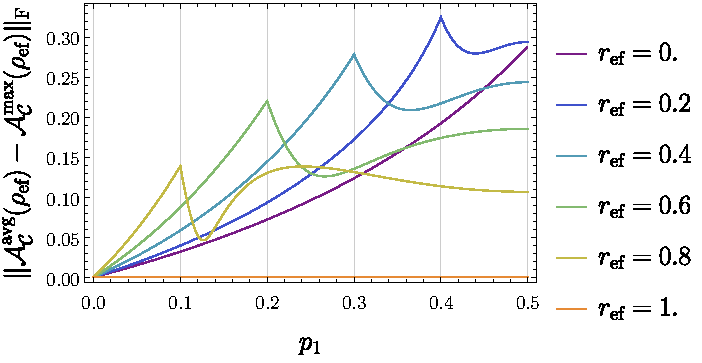
\includegraphics[width=1.\linewidth]{figures/avg_results/dist_maxent_avg_vs_p.pdf}
        \end{subfigure}%
        \begin{subfigure}{.45\textwidth}
          \centering
          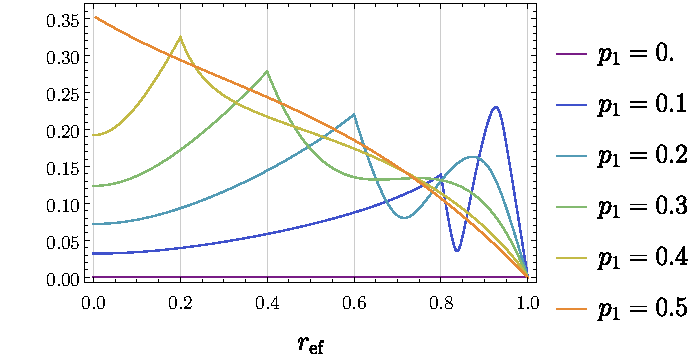
\includegraphics[width=1.\linewidth]{figures/avg_results/dist_maxent_avg_vs_z.pdf}
        \end{subfigure}
        \caption{Distancia de Frobenius entre asignaciones como función de $p_{1}$ para diferentes valores de $r_{z}$, y como función de $r_{z}$ para diferentes valores de $p_{1}$.}
    \end{figure}
\end{frame}

\begin{frame}{Discusión}
    La aplicación de asignación promedio no es fácilmente escalable a sistemas de $n$ qudits. Por otro lado, como se mostró en la sección \ref{sec:maxentcons}, utilizar el Principio de Máxima Entropía permite dichas extensiones de forma directa. Esto abre un camino directo a la obtención de resultados analíticos, cosa que se ha aprovechado. 
    
    En caso de no haber una razón para incluir únicamente estados puros en la definición de la aplicación de asignación promedio, esta restricción es tan arbitraria como considerar que todos los estados microscópicos compatibles con el estado efectivo son igualmente probables (suposición que también se hace). La elección de los estados a considerar, así como la medida sobre la que realizar la integración, son elementos de información que inyectan un sesgo a los resultados que puedan ser obtenibles. La aplicación de asignación de máxima entropía utiliza únicamente la información accesible al observador, y puede ser modificado para incluir nuevas restricciones. 
\end{frame}